\section{Background}
\label{sec:background}
Faults are difficult to detect before an executing system reaches a point of failure, as the first symptom of a fault is often system failure itself. While it is unrealistic to expect software to be fault-free, actions such as resetting the system, quarantining specific components, or minimizing damage from the fault can be taken. Autonomic systems, an extension of fault tolerant systems, attempt to detect, diagnose, and mitigate faults quickly. These systems are inspired by the autonomic nervous system in the human body that monitors and regulates vital  functions of the body such as heart rate, respiration rate, and digestion. Similarly, an autonomic computer system is able to monitor itself and its environment and adapt to complex changes. The goal of autonomic computing is to specify the desired state of a system using high-level objectives without detailing how to arrive at the state \cite{1160055,4061119,1301340}. By making intelligent decisions, autonomic systems free system administrators from low-level management and the intricacies of complex systems. Autonomic systems aim to be self-configuring, self-optimizing, self-healing, and self-protecting. These properties, collectively referred to as the self-* properties, are different views of the same self-man\-age\-ment property. For instance, a self-protecting system is ideally healing itself from faults while optimizing and reconfiguring itself to prevent other faults from reoccuring.

The heart of autonomic computing is anomaly detection, diagnosis, and mitigation. Autonomic systems perform 4 general tasks in a continuous closed loop: monitor components with the help of sensors, interpret the monitored data, create a repair plan for system adaptation, and execute this plan through effectors on the monitored system and its environment. This is the MAPE (Monitor, Analyze, Plan, Execute) loop \cite{1160055}. Figure~\ref{fig:mape} illustrates how an autonomic element uses this loop to manage a component.

\begin{figure}[tb]
  \centering
  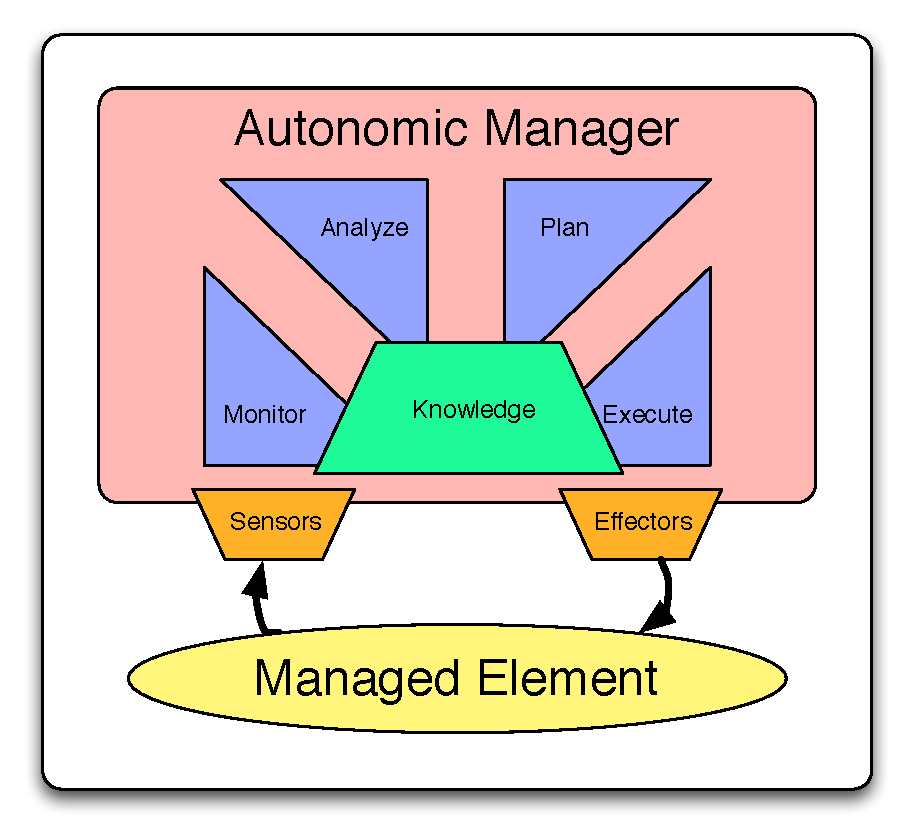
\includegraphics[width=\columnwidth]{images/mape}
  \caption{An autonomic element uses the MAPE control loop to monitor a component, analyze the its status with respect to a policy, plan how to meet the policy requirements, and execute a set of actions to do so.}
	\label{fig:mape}
\end{figure}

Autonomic approaches can be applied to many different types of systems, particularly when focusing on fault detection and mitigation. self-healing opearting systems \cite{DBLP:journals/ibmsj/AppavooHSWSKAEGGMORSX03,4351383} protect against bit-flips and other transient hardware faults, and are able to hot-swap components or firmware during runtime. At the application level, it is possible to monitor the architecture requirements of a system and detect when an architectural property (e.g. required connection bandwidth) falls outside of an acceptable threshold \cite{Garlan2004}. If an invariant is violated, it executes a strategy specifically designed to correct the violated invariant. The strategies can reinitialize components and reconfigure the system to recover from the violation and attempt to prevent the violation from reoccurring. However, the applied strategies are \emph{ad hoc} solutions, requiring developers and maintainers to understand and preempt the shortcomings of the system, in much the same way they would manually debug and repair the system.

\subsection{Fault Detection and Diagnosis}
\label{sub:fault_detection}

Previous approaches to the detection of software faults fall into two categories, signature-based and anomaly-based~\cite{al-nashif2008}. Signature-based methods detect faults by matching measurements to known fault signatures. These techniques are used in static fault-checking software such as the commercial antivirus software McAfee~\cite{Mcafee} and Symantec~\cite{symantec}, as well as network intrusion detection systems such as Snort~\cite{Roesch1999}  and Netstat~\cite{Vigna1999}. These techniques can also be used to detect recurring runtime faults~\cite{Brodie2005}.

Typically, anomaly-detection techniques begin by collecting sensor measurements of a normally behaving system. Then, they construct a representation of the monitored system and compare any future measurements against that representation. A common approach is to use metric correlations to quantify a monitored system. During detection, if the correlations between metrics becomes significantly different from the learned correlations, the system is classified to be in a faulty state~\cite{zhen2006,zhao2009,Cohen2004,Jiang2009}.

Once a fault is detected, it must be correctly diagnosed. Bayesian Network classifiers have been applied in several previous approaches to diagnosis using. Ghanbari et al. propose an approach to anomaly diagnosis based on Bayesian networks that are wholly or partially specified by a human user \cite{Ghanbari2008}. Tree augmented naive bayesian classifiers are the basis for software failure diagnosis in work by  Cohen et al.~\cite{Cohen2004}. Zhang et al. use ensembles of tree augmented naive Bayesian classifiers to diagnose faults.~\cite{Zhang2005}. Other classification techniques have been used to diagnose software faults. Chen et al.  offer an approach to the diagnosis of failures in large-scale Internet service systems using decision trees \cite{Chen2004}.  Duan et al.~\cite{Duan} propose an approach to diagnosis of software failures that uses active learning to minimize the number of data points that a human administrator must label.

In previous work it has been demonstrated that computational geometry can be used to effectively detect system faults at runtime\cite{stehle2010,shevertalov2010using}. The approach is split into a training phase, and a monitoring phase. During the training phase, the monitored system executes its normal behavior and runtime data is periodically collected from sensors monitoring the application, the operating system, and the hardware. Using these measurements, we can construct an $n$-dimensional convex hull whose enclosing space represents the normal execution of the monitored application, where $n$ is the number of distinct metrics used. Figure~\ref{fig:class_hulls} shows an example of a 2-dimensional convex hull.

\begin{figure}[tb]
  \centering
  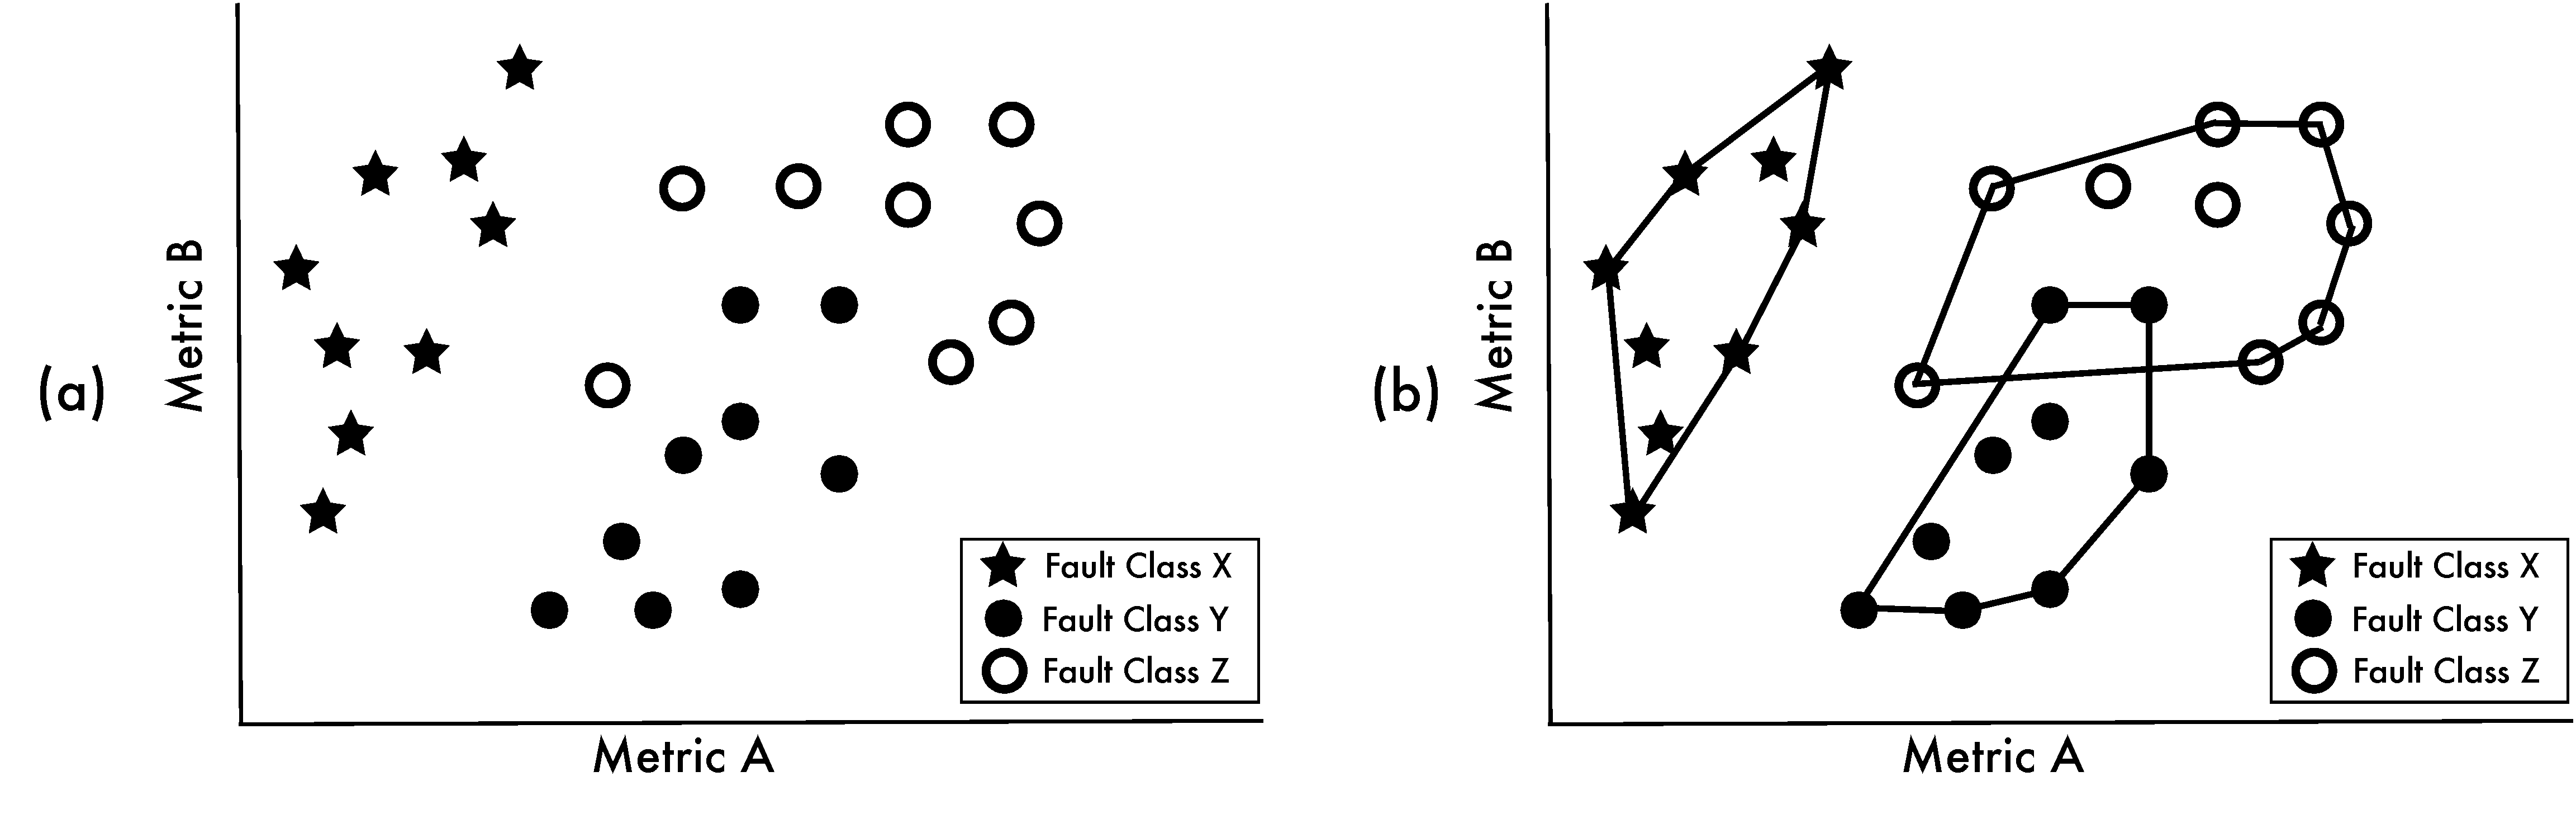
\includegraphics[width=\columnwidth]{images/class_hulls}
  \caption{Building convex hulls for the diagnosis of faults (a) sample points from normal operation and two fault classes (b) Points inside of the convex hulls are diagnosed as normal or one of the fault classes. Points outside of all hulls are diagnosed as unknown faults.}
  \label{fig:class_hulls}
\end{figure}

During the monitoring phase, if a measurement point falls outside of this enclosure, a fault is likely to have occurred. To properly mitigate the fault, the problem must be diagnosed \cite{6100108} and a viable mitigation selected. If measurement data is available for a set of known faults, then it is possible to construct hulls for individual faults, or classes of faults. During the monitoring phase, if a measurement falls within one of these fault hulls we can determine which fault is likely occurring and apply a mitigation.This approach is also capable of recognizing that an occurring fault is not a type of fault that it has been trained to recognize. Typical classification techniques, such as naive Bayes and voting feature intervals\cite{Demiroz1997}, require that every sample be assigned a class from a finite list of possible classes, which can cause drastic consequences if an incorrect mitigation is selected. Our approach allows Aniketos to recognize that a fault has occurred, but does not force Aniketos to label the fault as one of the faults that it has been trained to recognize. One of the most important features of a fault detection and diagnosis system is the ability to handle new faults.

\subsection{Fault Mitigation}
\label{sub:fault_mitigation}
To select the most appropriate mitigation to execute, mitigations must be evaluated based on their performance cost, impact on the system, reliability, and how they affect other mitigations. Given a set of faults and a set of mitigations, it is possible to intuitively and empiracally determine the best possible mitigation for a given fault.

However, not all information is known. Irreversible mitigations. Incorrect mitigations (catastrophic failure). Cascading effect.

When an anomaly occurs, multiple mitigations may be triggered at once. For instance, if a  hardware failure is detected on a host, all process should be migrated to another machine and diagnostic utilities should be run on the machine.